\section{Background}
\label{sec:bg}
The discretization of an infinite-dimensional problem leads to linear systems. The overall goal is not just to solve the linear system but to approximate the solution as closely as possible to its infinite-dimensional counterpart. Iterative approaches such as the Krylov subspace methods\nocite{liesen2019nla1} used for solving computationally expensive problems (read large sized matrices) often need the help of ``\emph{preconditioners}'' for optimal use of computational resources and for achieving desired convergence. Knowlegdge of the properties of the underlying PDE and discretization choices have been exploited to develop so-called ``operator'' preconditioners.\cite{hiptmair2006operator}.

Formally, this means given a continuous bijective linear operator $A : V \mapsto W$ on function spaces $V$ and $W$, and another isomorphism $B : W \mapsto V$, then $BA$ will provide an endomorphism of $V$. The discretization of $BA$ often leads to well-conditioned matrices. Therefore, the bounds of Krylov subspace iterations can become independent of mesh size.\\
For instance, in the present paper we consider the following problem setup
\begin{align}
  \label{eq:1}
& -\nabla\cdot(k(x)\nabla u) = f ,
& &x \in \Omega \\ \nonumber
&\hspace{1.5cm} u = 0, 
& &x \in \partial\Omega
\end{align}
and the corresponding eigenvalue problem 
\begin{align}
  \label{eq:2}
& -\nabla\cdot(k(x)\nabla u) = \lambda\Delta u ,
  & &x \in \Omega \\ \nonumber
&\hspace{1.5cm} u = 0, 
& &x \in \partial\Omega
\end{align}
for $f \in L^2(\Omega)$, and $k(x):\mathbb{R}^d \rightarrow \mathbb{R}$ \
$k(x)\geq \alpha > 0$; $x \in \Omega$. \\\\
Let $V_{h} \subset H_{0}^1(\Omega)$. In the corresponding finite element discretization of \eqref{eq:1} (and \eqref{eq:2}), we seek $u_{h} \in V_{h}$ such that,
\begin{align}
& \mathcal{A}_{h}u_{h} = f_{h} 
& & (\text{respectively} \mathcal{A}_{h}u_{h} = \lambda\mathcal{L}_{h}u_{h})
\end{align}
Finite dimensional subspace $V_{h}$ is spanned by piecewise polynomial basis functions \footnote{The authors assume Lagrangian polynomial basis in their study but note that the derived results are valid for any conforming approximation.} $\phi_1,\dots,\phi_N$ with the local supports. We then have $\mathcal{T}_i = \text{supp}(\phi_i)$, $i=1,\dots,N$.
Finally the matrix representations of $\mathcal{A}_{h}$ and $\mathcal{L}_{h}$ respectively become,
\begin{align}
  \label{eq:4}
[\mathbf{A}]_{i,j} &= \langle\mathcal{A}_{h}\phi_{j},\phi_{i}\rangle  =\int_{\Omega} \nabla\phi_i\cdot k\nabla\phi_j \\
[\mathbf{L}_{i,j} &= \langle\mathcal{A}_{h}\phi_{j},\phi_{i}\rangle = \int_{\Omega} \nabla\phi_i\cdot \nabla\phi_j
\end{align}

$i,j = 1,\dots,N$.

Now solving the system (eq.3) with Conjugate Gradients (CG), the corresponding energy norm in CG is known as, 
$$||x-x_j||_{\mathbf{A}}^2= \min_{p\in\mathcal{P}_j}||p(\mathbf{A})(x-x_0)||^2_{\mathbf{A}}$$, $j=1,2,...$
sing the spectral decomposition of the matrix $\mathbf{A}$ with eigenvalues $\lambda_1,\dots,\lambda_N$ with $v_1,\dots,v_N$ associated orthonormal eigenvectors,
We can rewrite (Ref. Section 2 \cite{gergelits2019laplacian}) it as, 

$$||x-x_j||_{\mathbf{A}}^2= ||r_0||^2\sum_{l=1}^N \omega_l \frac{(p_j^{CG}(\lambda_l))^2}{\lambda_l}$$
with,
$r_0 = b-\mathbf{A}x_0$, $\omega_l = (z,v_l)^2$, $l=1,\dots,N$ and $z=r_0/||r_0||$

The auhtors note the popular simplified relation of the CG bound dependent on the condition number $\kappa(\mathbf{A}) = \lambda_N/\lambda_1$
\begin{equation}
  \label{eq:cgbound}
  \frac{||x-x_j||_{\mathbf{A}}}{||x-x_0||_{\mathbf{A}}}\leq 2 \left(\frac{\sqrt{\kappa(\mathbf{A})-1}}{\sqrt{\kappa(\mathbf{A})+1}}\right)^j
\end{equation}
\clearpage
\section{Motivation}
\label{sec:mot}
\begin{figure}[ht]
  \centering
  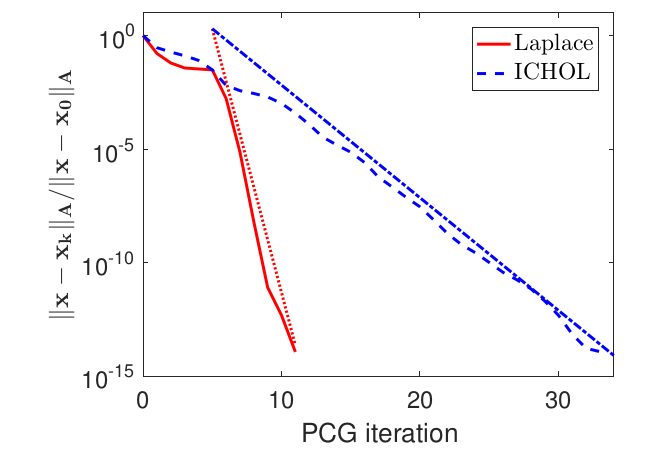
\includegraphics[scale=0.5]{explain.png}
  \caption{\label{fig:pcg}\cite[][Fig 1]{gergelits2019laplacian}The Laplacian operator preconditioning (solid line), is much more efficient than the incomplete Cholesky preconditioning (dashed line), despite the fact that the condition numbers are 161.54 and close to 16, respectively. (convergence based on example from \cite[]{gergelits2019laplacian}).}
\end{figure}

The authors, with the help of an example \parencite[Ref.][Section 2, An Example]{gergelits2019laplacian} illustrate the limitation with the bound mentioned in eqn. \eqref{eq:cgbound} to infer the convergence behaviour of the CG method. They take a boundary value problem similar to the system in eq. \eqref{eq:1} with $k(x)$ as a spatially varying piecewise constant function on individual subdomains. The rationale for such a particular choice seems to be the generation of an ill-conditioned matrix. Using the resulting linear FE discretization (eqns. \eqref{eq:4} \& (5)), the numerical solution $u$ to the system $\mathbf{Ax=b}$ is found by the preconditoned conjugate gradient (PCG) method. Laplacian operator based PCG is compared with an Incomplete Choleksy PCG. The authors observe from this experiment that the spectral condition number of the former is order of magnitude higher than the latter, eventhough the Laplace operator preconditioning demonstrated much faster convergence.\footnote{The authors compare the cost of individual preconditioned iterations not the overall computational cost of the problem.} (see \ref{fig:pcg}) They argue that the bound presented in \eqref{eq:cgbound} is often misconstrued. And the bound must be utilized by checking the spectrum of $\mathbf{A}$ and if it lies within $[\lambda_{1},\lambda_{N}]$. \cite{gergelits2014composite} is a recent paper that addresses this issue by arguing for composite convergence bounds. The authors motivate the present work by saying that a preconditioned Hermitian matrix with a \emph{favourable} distribution of the spectrum can lead to faster convergence rather than only focusing on minimizing the condition number. The primary aim of the paper is to prove the following conjecture based on the stated main results that we see in the next section \ref{sec:results}.

\begin{conjecture}
  \label{con:1}
  The spectrum of the discretized preconditioned operator $\mathbf{L}^{-1}\mathbf{A}$ can be approximated by the values of $k(x)$ of the supports of the FE basis functions in the problem setup eqn. \eqref{eq:2}
\end{conjecture}

\section{Main results}
\label{sec:results}
The two main results (Thm. 3.1 and Cor. 3.2) stated in the paper are first proven in \cite[][Section 3, Analysis]{gergelits2019laplacian} and then corresponding numerical experiments are given in \cite[][Section 4.1, Illust.]{gergelits2019laplacian}. Finally the authors present some additional corollary results and explain using the two main derived results the reason for faster convergence in the motivating example that was discussed before. Here we briefly outline the main results and the explanation of the motivating example.

\begin{theorem}{(pairing the eigenvalues and the intervals $k(\mathcal{T}_j)$,$ j=1,...,N$)}
  \label{thm:31}
Let $\lambda_1,...\lambda_N$ be the eigenvalues of $L^{-1}A$ where A and L are the conforming FEM global stiffness and mass matrices respectively and let $k(x)$ be bounded and piecewise continuous. Then there exists a (possibly non unique) permutation $\pi$ such that the eigenvalues of the matrix $L^{-1}A$ satisfy, 
$$\lambda_{\pi} \in k(\mathcal{T}_j)$$
\end{theorem}

\begin{figure}%
    \centering
    \subfloat[\centering sorted in ascending order ]{{\includegraphics[scale=0.25]{mendelsohn1} }}%
    \qquad
    \subfloat[\centering pairing $\pi$ computed  by  the  Dulmage-Mendelsohn decomposition  ofthe corresponding adjacency matrix $G$]{{\includegraphics[scale=0.35]{mendelsohn2} }}%
    \caption{Problem P4 from \cite{gergelits2019laplacian}}%
    \label{fig:example}%
\end{figure}

Theorem \ref{thm:31} constrains the locations of the individual eigenvalues of the matrix $\mathbf{L}^{-1}\mathbf{A}$ by a non unique pairing with the intervals $k(\mathcal{T}_j)$. The existence of a one-to-one pairing is represented by a bipartite graph (Ref eqn 3.13 in [1]). Lemma 3.3 and Corollary 3.4 are used to identify the groups of eigenvalues in any interval and then the Hall's theorem can be applied. We refer to the paper for the detailed proof. \\
The numerical examples presented in the paper for four different cases of $k(x,y)$
show the nodal values $k_{1},\dots,k_{N}$ and the corresponding eigenvalues of the matrix $\lambda_{1}, \dots, \lambda_{N}$ in close correspondence. Section 4.1 in [1] also explores potential pairings since the proof does not mention explicitly the permutation $\pi$ such that $\lambda_{\pi(i)} \in k(\mathcal(T_{i}))$. First the comparision is done with a simple ascending ordering of nodal $k(x,y)$ and $\lambda_{i}$ $\forall i \in {1,...,N}$. With the (P4) case mentioned in the paper (Ref. Fig \ref{fig:example}), some of the eigenvalues while sorted in increasing order did not lie inside the associated intervals. The authors then with the help of \emph{Dlmage-Mendelsohn decomposition} of the constructed adjacency matrix $G$ (see eqn 4.2, [1]) show an improvement in the positions of the eigenvalues. 

\begin{corollary}{(pairing the eigenvalues and the nodal values.)}
  \label{cor:32}
  
  Using the same notation and assumptions from Theorem 3.1, consider any point $\hat{x}_j$ such that $\hat{x}_j \in \mathcal{T}_j$. Then the associated eigenvalue $\lambda_{\pi(j)}$ of the matrix $L^{-1}A$ 
  $$|\lambda_{\pi(j)}-k(\hat{x}_j)| \leq \sup_{x \in \mathcal{T}_j}|k(x) - k(\hat{x}_j)|$$
  If in addition, $k(x) \in \mathcal{C}^{2}(\mathcal{T_{j}})$, then
  $$|\lambda_{\pi(j)}-k(\hat{x}_{j})|\leq \sup_{x \in \mathcal{T}_{j}}|k(x)-k(\hat{x}_{j})| \leq \hat{h}||\nabla k(\hat{x}_{j})|| + \frac{1}{2}\hat{h}^{2}\sup_{x \in mathcal{T}_{j}}||D^{2}k(x)||, \hspace{1cm} j=1,...,N$$
  where, $\hat{h}=diam(\mathcal{T}_{j})$ and $D^{2}k(x)$ is the second derivative of the function $k(x)$
\end{corollary}
With this result, it is shown in [[1], Section 4.1] the examples (P3) and (P4) are less accurate  pairings between $k(x)$ and $\lambda_{1},...,\lambda_{N}$ than (P1) and (P2) all given at a fixed mesh/resolution. The reason for (P3) to such a behaviour is due to the fact that the norm of the gradient of $k(x,y)=2^{7}(x^{7}+y^{7})$ is large in significant subregions. This is in agreement with Corollary 3.2. In (P4) the pairing is coarse, due to the usage of a discontinuous function. \\
\cite[][Section 4.2]{gergelits2019laplacian} also supports the results from Corollary 3.2. The four cases' estimated difference $|\lambda_{\pi(i)}-k(x_{i},y_{i})|$ scale linearly with the decrease in mesh size (read increase in number of degrees of freedom $N$). The authors show the flexibility of this result with two more examples: with local mesh refinement (Fig 11 in [1]) and with a sharp edged domain (Fig 12 in [1]). \cite[][Section 4.3]{gergelits2019laplacian}

\subsection{Explaination of accelerated convergence}
The behaviour of the convergence plot shown in Fig \ref{fig:pcg} was attributed to the structure of the spectrum of the preconditioned matrix system. The problem was set up such that a discontinuous step function in eigenvalues. (Ref. [1, Table 1]). Hence the two most populated eigenvalues ($1$ and $161.45$) contribute towards the CG iteration. The PCG converges using the effective condition number upper bound stated in [1, eqn. 4.3]. The authors explain that this is due to the fact that the Ritz values approximate the eigenvalues at the lower end of the spectrum closely. Hence, the convergence proceeds with a rate ignoring the approximated eigenvalues.
For a more detailed discussion, we refer to [1].

\section{Conclusion}
The authors have shown the eigenvalues of the preconditioned matrix $\mathbf{L}^{-1}{\mathbf{A}}$ lie in the resolution dependent intervals around the nodal values of the scalar coefficient function. They have shown a non-unique pairing of the eigenvalues and the coefficient function at the nodes. These two results then is utilized to explain the increased convergence rate of a Laplacian PCG eventhough the matrix is ill-conditioned.

\section{Open Questions}
Eventhough the authors present a compelling case for improvement in the performance of operator preconditioning applied to FEM discretized PDEs, a few questions remain.
\begin{itemize}
\item The study only considered second order elliptic PDEs. How do these results extend, if they can to \textbf{more general PDEs}? There has been an extension of these results to generalized second order differential operators. Refer \cite{gergelits2020generalized}
\item A second related question is with respect to the \textbf{discretization scheme}. Can the derived results be extended to alternative discretization schemes like the Finite Difference method.
\item The authors have considered the convergence performance with respect to the energy norm. What could be said about the \textbf{overall computational cost} of the Laplacian PCG? For instance, the calculation of $\mathbf{L}^{-1}\mathbf{A}$ with larger matrix sizes?  

\end{itemize}





%%% Local Variables:
%%% mode: latex
%%% TeX-master: "report"
%%% End:
